% =============================================================================
  % Cognotik DocOps — Live Demo Script
  % =============================================================================
  %
  % To render this file into a PDF, run:
  %
  %   pdflatex TOUR_2.tex
  %
  % Run it twice if you want the table of contents page references to resolve:
  %
  %   pdflatex TOUR_2.tex && pdflatex TOUR_2.tex
  %
  % Meow.
  % =============================================================================

  \documentclass[12pt, letterpaper]{article}

  % --- Packages ----------------------------------------------------------------
  \usepackage[utf8]{inputenc}
  \usepackage[T1]{fontenc}
  \usepackage{lmodern}
  \usepackage[margin=1in]{geometry}
  \usepackage{xcolor}
  \usepackage{titlesec}
  \usepackage{enumitem}
  \usepackage{fancyhdr}
  \usepackage{graphicx}
  \usepackage{hyperref}
  \usepackage{mdframed}
  \usepackage{fontawesome5}
  \usepackage{parskip}
  \usepackage{microtype}
  \usepackage{tocloft}
  \usepackage{tikz}

  % --- Colors ------------------------------------------------------------------
  \definecolor{cogblue}{HTML}{2563EB}
  \definecolor{cogdark}{HTML}{1E293B}
  \definecolor{coglight}{HTML}{F1F5F9}
  \definecolor{catpink}{HTML}{EC4899}
  \definecolor{catbg}{HTML}{FDF2F8}
  \definecolor{devbg}{HTML}{EFF6FF}
  \definecolor{stagebg}{HTML}{FEF9C3}
  \definecolor{notebg}{HTML}{F0FDF4}
  \definecolor{cardbg}{HTML}{F8FAFC}
  \definecolor{cardborder}{HTML}{CBD5E1}

  % --- Hyperref setup ----------------------------------------------------------
  \hypersetup{
    colorlinks=true,
    linkcolor=cogblue,
    urlcolor=cogblue,
    pdftitle={Cognotik DocOps -- Live Demo Script},
    pdfauthor={Cognotik},
    pdfsubject={Live Demo Script featuring a Developer and a Cat},
  }

  % --- Header / Footer ---------------------------------------------------------
  \pagestyle{fancy}
  \fancyhf{}
  \fancyhead[L]{\small\color{cogblue}\textbf{Cognotik DocOps} — Live Demo Script}
  \fancyhead[R]{\small\color{catpink}\faIcon{cat}\ Meow}
  \fancyfoot[C]{\thepage}
  \renewcommand{\headrulewidth}{0.4pt}
  \renewcommand{\footrulewidth}{0pt}

  % --- Section formatting ------------------------------------------------------
  \titleformat{\section}
    {\LARGE\bfseries\color{cogdark}}
    {\thesection}{1em}{}[\vspace{-0.3em}\textcolor{cogblue}{\rule{\textwidth}{1.5pt}}]

  \titleformat{\subsection}
    {\Large\bfseries\color{cogblue}}
    {\thesubsection}{1em}{}

  \titleformat{\subsubsection}
    {\large\bfseries\color{cogdark}}
    {\thesubsubsection}{1em}{}

  % --- Custom environments -----------------------------------------------------

  % Developer dialogue
  \newmdenv[
    backgroundcolor=devbg,
    linecolor=cogblue,
    linewidth=3pt,
    topline=false,
    bottomline=false,
    rightline=false,
    innerleftmargin=12pt,
    innerrightmargin=12pt,
    innertopmargin=10pt,
    innerbottommargin=10pt,
    skipabove=10pt,
    skipbelow=10pt,
  ]{developerbox}

  % Cat dialogue — extra large, extra readable, extra cat
  \newmdenv[
    backgroundcolor=catbg,
    linecolor=catpink,
    linewidth=3pt,
    topline=false,
    bottomline=false,
    rightline=false,
    innerleftmargin=12pt,
    innerrightmargin=12pt,
    innertopmargin=10pt,
    innerbottommargin=10pt,
    skipabove=10pt,
    skipbelow=10pt,
  ]{catbox}

  % Stage directions
  \newmdenv[
    backgroundcolor=stagebg,
    linecolor=black!20,
    linewidth=0.5pt,
    roundcorner=4pt,
    innerleftmargin=10pt,
    innerrightmargin=10pt,
    innertopmargin=6pt,
    innerbottommargin=6pt,
    skipabove=6pt,
    skipbelow=6pt,
  ]{stagebox}

  % Production / costume notes
  \newmdenv[
    backgroundcolor=notebg,
    linecolor=black!20,
    linewidth=0.5pt,
    roundcorner=4pt,
    innerleftmargin=10pt,
    innerrightmargin=10pt,
    innertopmargin=6pt,
    innerbottommargin=6pt,
    skipabove=6pt,
    skipbelow=6pt,
  ]{notebox}

  % Cue cards
  \newmdenv[
    backgroundcolor=cardbg,
    linecolor=cardborder,
    linewidth=1pt,
    roundcorner=6pt,
    innerleftmargin=14pt,
    innerrightmargin=14pt,
    innertopmargin=10pt,
    innerbottommargin=10pt,
    skipabove=12pt,
    skipbelow=12pt,
  ]{cuecard}

  % --- Convenience commands ----------------------------------------------------
  \newcommand{\dev}{\textbf{\color{cogblue}\faIcon{laptop-code}\ Developer:}}
  \newcommand{\cat}{\textbf{\color{catpink}\faIcon{cat}\ Cat:}}
  \newcommand{\stage}[1]{%
    \begin{stagebox}%
      \textit{\color{black!60}#1}%
    \end{stagebox}%
  }

  % =============================================================================
  \begin{document}

  % --- Title Page --------------------------------------------------------------
  \begin{titlepage}
    \centering
    \vspace*{2cm}

    \begin{tikzpicture}
      \node[fill=catpink!10, rounded corners=20pt, inner sep=20pt] {
        \begin{minipage}{0.7\textwidth}
          \centering
          {\fontsize{48}{52}\selectfont \faIcon{cat}}\\[12pt]
          {\Huge\bfseries\color{cogdark} Cognotik DocOps}\\[8pt]
          {\LARGE\color{cogblue} Live Demo Script}\\[16pt]
          {\large\color{cogdark}
            A combined presenter script for the Cognotik DocOps live demo.\\[6pt]
            \textit{Featuring the Developer and a very special\\co-presenter: the Cat.}
          }
        \end{minipage}
      };
    \end{tikzpicture}

    \vfill

    {\large\color{black!50} \faIcon{rocket}\ Press a button. Get a thing. Meow.}

    \vspace{2cm}
  \end{titlepage}

  % --- Table of Contents -------------------------------------------------------
  \tableofcontents
  \newpage

  % --- How to Use This Script --------------------------------------------------
  \section*{How to Use This Script}
  \addcontentsline{toc}{section}{How to Use This Script}

  This is a single script for both presenters. The \textbf{Developer} delivers the
  technical content and operates the computer. The \textbf{Cat} (your daughter, in
  her cat mask) delivers the punchlines, the summaries, and the proof that it all
  actually works.

  Lines marked \dev{} are yours. Lines marked \cat{} are hers.
  Stage directions are in \textit{[brackets]} on a yellow background.

  \begin{notebox}
    \faIcon{mask}\ \textbf{Costume note:} Cat mask required. Cat ears encouraged.
    A tail is a power move.
  \end{notebox}

  \begin{notebox}
    \faIcon{film}\ \textbf{Production note:} If the Cat goes off-script, that's fine.
    That's very cat behavior. Do not attempt to correct the Cat. The Cat knows what
    she's doing.
  \end{notebox}

  \newpage

  % =============================================================================
  %  PART ONE: OPENING & OVERVIEW
  % =============================================================================
  \section{Part One: Opening \& Overview}

  % ---------------------------------------------------------------------------
  \subsection{Scene 1 — The Grand Entrance}

  \stage{Developer is at the front of the room. The Cat enters — or has been
  sitting quietly and now stands up.}

  \begin{developerbox}
    \dev{} Before I get started, I need to introduce my co-presenter for today.
  \end{developerbox}

  \begin{catbox}
    \cat{} \large Meow.

    \medskip
    {\large\textit{(pause for effect)}}

    \medskip
    {\large
    I am a cat. I do not know how to code. I do not know what a pipeline is.
    I do not even know what a computer is, really. I am a cat.}

    \medskip
    {\large\textit{(very serious face)}}

    \medskip
    {\large
    But I can use Cognotik. Because it is \textbf{THAT} easy.}

    \medskip
    {\large Meow.}

    \medskip
    {\large\textit{(sits back down with great dignity)}}
  \end{catbox}

  \begin{developerbox}
    \dev{} She's not wrong. And that's actually the whole point of what I'm going
    to show you today. So let's get into it.
  \end{developerbox}

  % ---------------------------------------------------------------------------
  \subsection{Scene 2 — What Is Cognotik DocOps?}

  \begin{developerbox}
    \dev{} Here's the problem we built Cognotik to solve. Everyone has ideas —
    articles they want to write, apps they want to build, tasks they want to
    automate. And there's always something in the way. You don't know JavaScript.
    You don't have time to learn shell scripting. Your notes have been sitting in
    a folder for six months.

    \medskip
    Cognotik DocOps is a platform that closes that gap. You describe what you want
    in plain language. You press a button. The AI does the work — and you can watch
    it happen in real time.

    \medskip
    It's a suite of applications, each built for a different kind of work. But they
    all follow the same pattern: you bring the idea, the platform handles the
    execution.

    \medskip
    Let me ask my co-presenter to summarize.
  \end{developerbox}

  \begin{catbox}
    \cat{} \large Okay. So.

    \medskip
    {\large You have an idea.}

    \medskip
    {\large\textit{(holds up one finger)}}

    \medskip
    {\large You type the idea.}

    \medskip
    {\large\textit{(holds up two fingers)}}

    \medskip
    {\large You press a button.}

    \medskip
    {\large\textit{(holds up three fingers — or tries to, gives up)}}

    \medskip
    {\large The computer does the rest.}

    \medskip
    {\large\textit{(shrugs)}}

    \medskip
    {\large That is the whole thing. That is Cognotik.}

    \medskip
    {\large Even I can do that, and I am a cat. Meow.}
  \end{catbox}

  % ---------------------------------------------------------------------------
  \subsection{Scene 3a — What Makes This Different}

  \begin{developerbox}
    \dev{} Now, there are a lot of AI tools out there. You've probably used some
    of them. You type a prompt, you get an answer, and you hope it's good. If it's
    not — well, you try again and hope harder.

    \medskip
    Cognotik works differently, and I want to explain why, because it matters for
    everything you're about to see.

    \medskip
    First: \textbf{everything is visible.} When a pipeline runs, you can watch the
    AI think. You can open a live session link and see the tokens appearing in real
    time. Every intermediate step produces a file you can read. There's no black
    box. If something goes wrong, you can see exactly where and why.

    \medskip
    Second: \textbf{everything is structured.} Instead of one big prompt, Cognotik
    breaks work into a sequence of steps — a pipeline. Each step has a clear input
    and a clear output, and each step builds on the last. That's why the results
    are more coherent than what you get from a single prompt. The AI is thinking in
    stages, and staged thinking produces better work.

    \medskip
    Third: \textbf{everything is iterative.} The first run is almost never the
    final run. And that's fine — that's how it's designed. You refine your input,
    you re-run, and the outputs get better. The whole system is built around the
    idea that good work comes from multiple passes, not one lucky shot.

    \medskip
    And here's the part that ties it all together: \textbf{everything lives in
    files.} Your inputs, your outputs, the status of every operation — it's all
    just files in a directory. Nothing is hidden in a database. You can download
    your whole session as a ZIP and read every artifact on your laptop. That means
    everything is resumable, everything is portable, and everything is auditable.

    \medskip
    So when I say ``you can watch it work'' — I mean that literally. And when I say
    ``you can trust the output'' — I mean you can verify it yourself, step by step.

    \medskip
    That's the foundation. Now let me show you what's built on top of it.
  \end{developerbox}

  % ---------------------------------------------------------------------------
  \subsection{Scene 3b — Getting Started}

  \begin{developerbox}
    \dev{} Before we dive into the apps, let me quickly show you how you'd
    actually get up and running.

    \medskip
    First, you go to \textbf{cognotik.com} and click the download link for your
    operating system. It's available for Mac, Windows, and Linux. You install it
    like any other application, and when you open it, it starts a local server on
    your machine.

    \medskip
    Next — and I'll gloss over this part — you configure your API keys for
    whichever AI provider you want to use. OpenAI, Anthropic, Google — the
    platform supports multiple providers. You paste in your key, and you're done.
    That's the only configuration step.

    \medskip
    Once that's set up, you open your browser to the localhost homepage, and you'll
    see all the available applications listed right there. You click one, and
    you're working. That's it — no cloud account, no subscription portal, no
    deployment step. It runs on your machine, your data stays on your machine.

    \medskip
    Now, for the purposes of this tour, I'm not going to run everything live from
    a local install — that would involve a lot of waiting for pipelines to
    complete. Instead, we're going to go back to the \textbf{cognotik.com} website,
    which has \textbf{archived sessions} for each app. These are real outputs from
    real pipeline runs, preserved so you can explore every step and every artifact.
    Everything you're about to see is exactly what you'd get running it yourself.
  \end{developerbox}

  \begin{catbox}
    \cat{} \large So\ldots

    \medskip
    {\large You download it. You put in a key. You open it.}

    \medskip
    {\large\textit{(counting on fingers)}}

    \medskip
    {\large Three things. And then you have all the apps.}

    \medskip
    {\large\textit{(to audience)}}

    \medskip
    {\large We are looking at the website version today because waiting is boring.}

    \medskip
    {\large Meow.}
  \end{catbox}

  \newpage

  % =============================================================================
  %  PART TWO: THE APPLICATIONS
  % =============================================================================
  \section{Part Two: The Applications}

  % ---------------------------------------------------------------------------
  \subsection{Scene 4 — The Philosophical Calculator}

  \begin{catbox}
    \cat{} \large The next app is for thinking.

    \medskip
    {\large Cats think a lot. Mostly about birds. And naps.}

    \medskip
    {\large But if I had a big important idea — like, what if there were
    \textbf{MORE} birds — I would put it in here, and the computer would make it
    into a whole essay.}

    \medskip
    {\large With arguments and everything.}

    \medskip
    {\large\textit{(nodding slowly)}}

    \medskip
    {\large Very impressive. Meow.}
  \end{catbox}

  \begin{developerbox}
    \dev{} She's basically right. The Philosophical Calculator is where you start
    when you have raw material — notes, transcripts, half-formed ideas — and you
    want to turn it into something rigorous.

    \medskip
    You drop in your notes. The platform summarizes them, drafts an article, and
    then runs your draft through a set of analytical lenses — dialectical,
    Socratic, game-theoretic, persuasive, narrative, and more. Each pass deepens
    the content without overwriting your voice. Then it weaves all those insights
    back into a single, richer piece.

    \medskip
    Think of it as having a panel of brilliant advisors who each read your draft
    and hand back a different kind of feedback. And because it's a pipeline — not a
    single prompt — each analytical pass builds on the ones before it. The result
    is qualitatively different from what you'd get asking a chatbot to ``make this
    better.''

    \medskip
    Your notes are always the source of truth. The system refines. It doesn't
    replace.
  \end{developerbox}

  % ---------------------------------------------------------------------------
  \subsection{Scene 5 — The Webapp Builder}

  \begin{catbox}
    \cat{} \large This one builds websites.

    \medskip
    {\large I cannot build a website. I have paws.}

    \medskip
    {\large\textit{(holds up paws as evidence)}}

    \medskip
    {\large But I can \textbf{DESCRIBE} a website. I can say: I want a website
    about cats. With pictures of cats. And a button that says ``meow'' when you
    press it.}

    \medskip
    {\large And then\ldots}

    \medskip
    {\large\textit{(snaps fingers — or tries to)}}

    \medskip
    {\large \ldots website.}

    \medskip
    {\large Meow.}
  \end{catbox}

  \begin{developerbox}
    \dev{} The Webapp Builder takes a plain-language description and produces a
    working web application in a single pipeline run. You describe the purpose, the
    users, the features, the look and feel. The pipeline plans the architecture,
    generates design documents, and implements all the code. An embedded preview
    shows you the result right in the interface.

    \medskip
    The more specific you are, the better the output. Mention UI patterns by name —
    ``Kanban board,'' ``sidebar navigation.'' Specify constraints — ``vanilla JS
    only,'' ``dark theme,'' ``mobile-first.'' And if the first result isn't quite
    right, you refine your description and run it again. That iterative loop I
    mentioned earlier — this is where you really feel it.

    \medskip
    This is the tool that turns ``I wish I had an app that\ldots'' into an actual
    app you can click on.
  \end{developerbox}

  % ---------------------------------------------------------------------------
  \subsection{Scene 6 — The System Wizard}

  \begin{catbox}
    \cat{} \large This one writes\ldots\ shell scripts.

    \medskip
    {\large\textit{(long pause)}}

    \medskip
    {\large I do not know what a shell script is.}

    \medskip
    {\large\textit{(another pause)}}

    \medskip
    {\large But I know what a shell is. You find them at the beach.}

    \medskip
    {\large\textit{(thinking very hard)}}

    \medskip
    {\large Anyway. You tell it what you want to happen on your computer, and it
    writes the script, and runs it, and if it breaks, it fixes itself.}

    \medskip
    {\large I wish I could fix myself when I break things.}

    \medskip
    {\large\textit{(looks at something offscreen)}}

    \medskip
    {\large \ldots The vase is fine. Meow.}
  \end{catbox}

  \begin{developerbox}
    \dev{} The System Wizard handles the operational side of things. You describe a
    task — ``set up a Python virtual environment,'' ``find all PNGs larger than 5MB
    and compress them'' — and it writes a shell script, runs it, and if something
    goes wrong, it reads the error output, patches the script, and tries again.

    \medskip
    You can watch the whole process in the Results tab. The generated script, the
    execution log, your original goal — it's all visible. And that auto-fix loop is
    a great example of why the pipeline model matters. A single prompt can write
    you a script. But a pipeline can write a script, test it, read the failure, and
    fix it — automatically. That's a fundamentally different level of reliability.
  \end{developerbox}

  % ---------------------------------------------------------------------------
  \subsection{Scene 7 — Omega: The App Generator}

  \begin{catbox}
    \cat{} \large Okay. This is the big one.

    \medskip
    {\large\textit{(stands up straighter)}}

    \medskip
    {\large This app\ldots\ makes \textbf{OTHER} apps.}

    \medskip
    {\large\textit{(lets that sink in)}}

    \medskip
    {\large You describe the app you want. And it \textbf{BUILDS} it. The whole
    thing.}

    \medskip
    {\large So if I wanted an app that is just\ldots\ a button that says
    meow\ldots}

    \medskip
    {\large I could make that.}

    \medskip
    {\large\textit{(very quietly, to self)}}

    \medskip
    {\large I am going to make that.}

    \medskip
    {\large\textit{(to audience)}}

    \medskip
    {\large Meow.}
  \end{catbox}

  \begin{developerbox}
    \dev{} Omega is the meta-application. It generates other DocOps applications
    from a plain-language description. You describe what you want — a pitch deck
    generator, a research assistant, a content repurposing tool — and Omega
    produces the requirements document, the full AI pipeline, and a complete
    single-page UI.

    \medskip
    It also has an iteration tab where you can describe changes — ``add a new
    analysis step,'' ``change the layout to tabs'' — and the AI applies targeted
    updates. There's even built-in Git integration so you can commit working
    versions before you experiment.

    \medskip
    This is the logical endpoint of the whole platform's philosophy. If every other
    app turns your ideas into outputs, Omega turns your ideas into tools. The right
    pipeline for your work might not be one of the apps I've shown you today. It
    might be something you design yourself. Omega makes that possible.
  \end{developerbox}

  \newpage

  % =============================================================================
  %  PART THREE: THE FULL APP WALKTHROUGH
  % =============================================================================
  \section{Part Three: The Full App Walkthrough — Comic Serial Generator}

  \begin{center}
    \textit{\large This is the Cat's big moment. A complete, step-by-step
    walkthrough of one app, narrated by the Cat. The Developer operates the
    computer.}
  \end{center}

  % ---------------------------------------------------------------------------
  \subsection{Scene 8 — The Comic Serial Generator}

  \stage{Developer opens the Comic Serial Generator in the browser.}

  \begin{catbox}
    \cat{} \large Okay. I am going to show you this one myself.

    \medskip
    {\large This app takes any idea — \textbf{ANY} idea — and turns it into a
    comic book. A whole series. With characters. And a story. And pictures
    described in words.}

    \medskip
    {\large\textit{(to Developer)}}

    \medskip
    {\large Can you open it please?}

    \medskip
    {\large\textit{[Developer opens the app]}}

    \medskip
    {\large Thank you.}

    \medskip
    {\large\textit{(to audience)}}

    \medskip
    {\large See? I told him what I wanted and he did it. Very easy.}
  \end{catbox}

  % --- Step 1 ------------------------------------------------------------------
  \subsubsection{Step 1: The Idea}

  \stage{Developer clicks into the input area. The Cat dictates.}

  \begin{catbox}
    \cat{} \large So. First you need an idea.

    \medskip
    {\large My idea is: a cat who discovers that the red dot from the laser pointer
    is actually a signal from an alien civilization trying to make first contact,
    and the cat is the only one who can decode it.}

    \medskip
    {\large\textit{(pause)}}

    \medskip
    {\large I have been thinking about this for a while.}

    \medskip
    {\large\textit{(to Developer)}}

    \medskip
    {\large Type that in please.}

    \medskip
    {\large\textit{[Developer types the idea into the input area]}}

    \medskip
    {\large Good. Now — you see this box? This is where the idea goes. You
    just\ldots\ write it. In normal words. No code. No special language.}

    \medskip
    {\large Just words. Even a cat can write words.}

    \medskip
    {\large\textit{(beat)}}

    \medskip
    {\large Well. I am dictating. But still.}
  \end{catbox}

  \begin{developerbox}
    \dev{} And this is a good moment to point out — the input here is just plain
    text. That's true across the whole suite. You don't need to learn a special
    syntax or configure anything. You describe what you want, and the pipeline
    takes it from there.
  \end{developerbox}

  % --- Step 2 ------------------------------------------------------------------
  \subsubsection{Step 2: Generate Episode One}

  \stage{Developer clicks the ``Generate'' button.}

  \begin{catbox}
    \cat{} \large Now we press the button.

    \medskip
    {\large\textit{(watches screen)}}

    \medskip
    {\large And now\ldots\ we wait.}

    \medskip
    {\large\textit{(sits very still, watching)}}

    \medskip
    {\large You can see it working. Right there. Those words appearing — that is
    the AI writing the comic. In real time.}

    \medskip
    {\large\textit{(leans forward)}}

    \medskip
    {\large It is making characters. It is deciding what they look like. It is
    figuring out the story.}

    \medskip
    {\large\textit{(whispers)}}

    \medskip
    {\large It is doing a lot of work very fast.}

    \medskip
    {\large\textit{(sits back)}}

    \medskip
    {\large I did not do any of that work. I just had the idea.}

    \medskip
    {\large Meow.}
  \end{catbox}

  \begin{developerbox}
    \dev{} What you're seeing right now is the live session monitoring I mentioned
    earlier. The AI is working through the pipeline step by step, and every token
    is visible as it's generated. This is what I mean when I say the process is
    transparent. You're not waiting for a result to appear out of nowhere — you're
    watching it being built.
  \end{developerbox}

  % --- Step 3 ------------------------------------------------------------------
  \subsubsection{Step 3: Reading the Result}

  \stage{The first episode has generated. Developer scrolls through it.}

  \begin{catbox}
    \cat{} \large Okay! Look at this.

    \medskip
    {\large Episode One. It has a title. It has a main character —}

    \medskip
    {\large\textit{(reading)}}

    \medskip
    {\large — oh, the cat's name is Captain Whiskers. Good name. I approve.}

    \medskip
    {\large It has a setting. It has dialogue. It has panel descriptions.}

    \medskip
    {\large\textit{(to audience)}}

    \medskip
    {\large I did not write any of this. I said: cat, laser pointer, aliens.}

    \medskip
    {\large And it wrote\ldots\ all of this.}

    \medskip
    {\large\textit{(gesturing at screen)}}

    \medskip
    {\large This is a whole comic book issue. From my idea.}

    \medskip
    {\large\textit{(nodding slowly)}}

    \medskip
    {\large Very good computer.}
  \end{catbox}

  % --- Step 4 ------------------------------------------------------------------
  \subsubsection{Step 4: The Sequel}

  \stage{Developer clicks to generate Episode 2.}

  \begin{catbox}
    \cat{} \large But wait. It gets better.

    \medskip
    {\large We can make \textbf{MORE}.}

    \medskip
    {\large See this button? This makes the next episode. And the next episode will
    \textbf{REMEMBER} everything from episode one. The characters. The story. Where
    we left off.}

    \medskip
    {\large It is not starting over. It is continuing.}

    \medskip
    {\large\textit{(points at Developer)}}

    \medskip
    {\large Go ahead.}

    \medskip
    {\large\textit{[Developer clicks]}}

    \medskip
    {\large\textit{(waits)}}

    \medskip
    {\large See? Episode two. Captain Whiskers is back. The aliens are back. The
    story keeps going.}

    \medskip
    {\large\textit{(to audience)}}

    \medskip
    {\large I could make five of these. Ten. A whole season.}

    \medskip
    {\large\textit{(quietly)}}

    \medskip
    {\large I might do that later.}
  \end{catbox}

  \begin{developerbox}
    \dev{} This is the iterative model in action. Each episode builds on the
    previous one — the pipeline carries context forward. And there's also a batch
    option if you want to generate a whole arc at once. The point is, you're not
    starting from scratch every time. The system remembers, and the work compounds.
  \end{developerbox}

  % --- Step 5 ------------------------------------------------------------------
  \subsubsection{Step 5: The Wrap-Up}

  \begin{catbox}
    \cat{} \large So. To summarize.

    \medskip
    {\large I had an idea. I typed the idea — well, I said the idea out loud and a
    human typed it, but that is fine, delegation is a skill —}

    \medskip
    {\large I pressed a button.}

    \medskip
    {\large And now I have a comic book series.}

    \medskip
    {\large\textit{(spreads paws wide)}}

    \medskip
    {\large About a cat. Who is a hero. Saving the world from aliens.}

    \medskip
    {\large\textit{(very seriously)}}

    \medskip
    {\large This is the most important comic series ever made.}

    \medskip
    {\large And it took about two minutes.}

    \medskip
    {\large\textit{(to audience)}}

    \medskip
    {\large I am a cat. I cannot code. I cannot do math. I knocked a glass of
    water off the table this morning on purpose.}

    \medskip
    {\large And I just made a comic book series.}

    \medskip
    {\large\textit{(pause)}}

    \medskip
    {\large Meow.}
  \end{catbox}

  \newpage

  % =============================================================================
  %  PART FOUR: CLOSING
  % =============================================================================
  \section{Part Four: Closing}

  % ---------------------------------------------------------------------------
  \subsection{Scene 9 — The Final Word}

  \begin{developerbox}
    \dev{} And that's the Cognotik DocOps suite. Let me do a quick recap of what
    ties it all together.

    \medskip
    Every app in the suite works the same way: plain-language input, structured AI
    pipeline, visible output. You can watch the AI work in real time. Everything
    lives in files you can read and inspect. And everything is designed for
    iteration — you refine, you re-run, you improve.

    \medskip
    The Philosophical Calculator sharpens your thinking. The Webapp Builder turns
    descriptions into working apps. The Comic Serial Generator turns ideas into
    stories. The System Wizard automates tasks and fixes its own mistakes. And
    Omega lets you build your own tools on top of the same platform.

    \medskip
    The common thread is this: the quality of your ideas — not your technical
    background — determines what you can build. That's what the platform is for.
    That's what makes it different.

    \medskip
    But I think my co-presenter has some closing thoughts.
  \end{developerbox}

  \begin{catbox}
    \cat{} \large Yes. Thank you.

    \medskip
    {\large\textit{(steps forward)}}

    \medskip
    {\large You have just seen: a writing tool. A website builder. A comic maker.
    A script fixer. An app that makes apps.}

    \medskip
    {\large All of them work the same way.}

    \medskip
    {\large You have an idea. You describe the idea. You press a button.}

    \medskip
    {\large\textit{(holds up one paw)}}

    \medskip
    {\large That is it.}

    \medskip
    {\large No coding. No configuration. No special knowledge required.}

    \medskip
    {\large\textit{(gestures to self)}}

    \medskip
    {\Large\bfseries I am seven years old.}

    \medskip
    {\Large\bfseries I am wearing a cat mask.}

    \medskip
    {\Large\bfseries I made a comic book today.}

    \medskip
    {\large\textit{(long pause)}}

    \medskip
    {\Large If you cannot figure out Cognotik\ldots}

    \medskip
    {\large\textit{(looks at audience)}}

    \medskip
    {\Large \ldots I do not know what to tell you.}

    \medskip
    {\large\textit{(sits down with finality)}}

    \medskip
    {\Large\bfseries Meow.}
  \end{catbox}

  \begin{developerbox}
    \dev{} She's right. Thank you all. We'll be around for questions.
  \end{developerbox}

  \newpage

  % =============================================================================
  %  APPENDIX: CUE CARDS FOR THE CAT
  % =============================================================================
  \section{Appendix: Quick-Reference Cue Cards for the Cat}

  \begin{center}
    \textit{Print these out and cut them apart. Hand to Cat before the demo.}
  \end{center}

  \bigskip

  % --- Card 1 ------------------------------------------------------------------
  \begin{cuecard}
    \begin{center}
      {\Large \faIcon{cat}\ \textbf{\color{catpink}Card 1 — ENTRANCE}}
    \end{center}
    \medskip
    {\large
    ``Meow. I am a cat. I cannot code.
    But I can use Cognotik. Because it is THAT easy. Meow.''}
  \end{cuecard}

  % --- Card 2 ------------------------------------------------------------------
  \begin{cuecard}
    \begin{center}
      {\Large \faIcon{cat}\ \textbf{\color{catpink}Card 2 — SUMMARY}}
    \end{center}
    \medskip
    {\large
    ``You have an idea. You type it. You press a button.
    The computer does the rest. Even I can do that. Meow.''}
  \end{cuecard}

  % --- Card 3 ------------------------------------------------------------------
  \begin{cuecard}
    \begin{center}
      {\Large \faIcon{cat}\ \textbf{\color{catpink}Card 3 — PHILOSOPHICAL CALCULATOR}}
    \end{center}
    \medskip
    {\large
    ``This one is for thinking. Cats think a lot.
    Mostly about birds. But this makes your ideas into essays. Meow.''}
  \end{cuecard}

  % --- Card 4 ------------------------------------------------------------------
  \begin{cuecard}
    \begin{center}
      {\Large \faIcon{cat}\ \textbf{\color{catpink}Card 4 — WEBAPP BUILDER}}
    \end{center}
    \medskip
    {\large
    ``This builds websites. I have paws. But I can describe a website.
    And then — website. Meow.''}
  \end{cuecard}

  % --- Card 5 ------------------------------------------------------------------
  \begin{cuecard}
    \begin{center}
      {\Large \faIcon{cat}\ \textbf{\color{catpink}Card 5 — SYSTEM WIZARD}}
    \end{center}
    \medskip
    {\large
    ``This writes shell scripts. I don't know what those are.
    But it fixes itself when it breaks. I wish I could do that.
    The vase is fine. Meow.''}
  \end{cuecard}

  % --- Card 6 ------------------------------------------------------------------
  \begin{cuecard}
    \begin{center}
      {\Large \faIcon{cat}\ \textbf{\color{catpink}Card 6 — OMEGA}}
    \end{center}
    \medskip
    {\large
    ``This app makes OTHER apps. I am going to make a meow button.
    Meow.''}
  \end{cuecard}

  % --- Card 7 ------------------------------------------------------------------
  \begin{cuecard}
    \begin{center}
      {\Large \faIcon{cat}\ \textbf{\color{catpink}Card 7 — COMIC WALKTHROUGH}}
    \end{center}
    \medskip
    {\large
    ``I had an idea. I pressed a button. Now I have a comic book series.
    I am a cat and I did that. Meow.''}
  \end{cuecard}

  % --- Card 8 ------------------------------------------------------------------
  \begin{cuecard}
    \begin{center}
      {\Large \faIcon{cat}\ \textbf{\color{catpink}Card 8 — CLOSING}}
    \end{center}
    \medskip
    {\large
    ``I am seven. I am wearing a cat mask. I made a comic book today.
    If you cannot figure out Cognotik, I do not know what to tell you. Meow.''}
  \end{cuecard}

  \vfill

  \begin{center}
    \textit{\color{catpink}\Large\faIcon{cat}\ End of TOUR\_2 — Meow.\ \faIcon{cat}}
  \end{center}

  \end{document}